\chapter{General Discussion}\thumbforchapter
\newpage

\noindent
All cells in our body contain the same DNA, yet the cells in our liver express a completely different set of genes than the cells in our heart. Gene expression regulation is the mechanism that controls the activation and repression of genes in the genome. The spatial and temporal control of gene regulation is an essential part of (embryonic) development. Moreover, genes and their spatio-temporal expression patterns and regulation are remarkably conserved between species.

In this thesis, I studied gene expression regulation from an evolutionary-developmental point of view. I first discussed three recommendations for gene regulatory network inference in development; multi-omics data, single-cell sequencing, and artificial neural nets (\textbf{Chapter 2}). Next, I presented seq2science, a preprocessing workflow for functional genomics analysis (\textbf{Chapter 3}). This chapter is followed by a description of how the definition of the phylotypic stage is ambiguous and how this ambiguity leads to the development of missing statistical controls. Applying these new controls to previous studies exposes flaws in the methodology and the subsequent interpretation of their results (\textbf{Chapters 4 and 5}). Finally, in \textbf{Chapter 6}, I presented a novel method to infer transcription factor activity based on single-cell transcriptomic data. Here I present my final concluding remarks.

\section{Inferring gene regulatory networks}

Gene regulatory network inference is the computational and statistical approach to decipher the regulatory interactions between genes. Understanding how certain gene products, for instance, transcription factors, regulate the expression of other genes helps with gaining a fundamental understanding of cellular processes. It has become a standard analysis step in most (single-cell) studies, however, the field seems to dismiss the fact that the inferred networks perform barely any better than random networks\cite{McCalla_2021,Chen_2018,Pratapa_2020}. In \textbf{Chapter 2} I discuss three (potential) improvements over "traditional" gene regulatory network inference; the inclusion of multi-omics data, single-cell sequencing, and artificial neural networks.

As a first recommendation, I suggest the inclusion of multiple sequencing modalities. Historically, gene regulatory networks have mainly been inferred based on transcriptomic data alone. Apart from the issue that these networks perform poorly\cite{McCalla_2021,Chen_2018,Pratapa_2020}, there is the fundamental issue of using transcripts both as input and as output in these models. Transcript abundance is the result of transcription regulation and degradation. Transcripts, however, are typically not responsible for signal transduction, chromatin remodeling, translation, and transcription regulation and degradation. The protein product synthesized from these transcripts, however, is responsible for these types of regulation and is assumed to correlate closely with transcript abundance. The correlation coefficient between transcript and protein, however, ranges between 0.3-0.4\cite{Fortelny2017,Franks2017}, with transcript abundance thus approximately explaining only between 0.09-0.16 of the variance of protein abundance. Similarly, in \textbf{Chapter 6} I show a poor correlation between transcription factor expression level and its motif activity. High-throughput proteomics is more costly than sequencing data and lacks its accuracy, with single-cell proteomics lagging behind single-cell transcriptomic and (epi)genomic techniques\cite{Bennett2023}. More accessible and accurate metrics for gene regulation are epigenomic assays that measure genome accessibility and histone modifications\cite{Xu_2020,Kamal_2021,Aibar_2017}, which in turn improve the performance of these models. Ideally, future GRN inference methods include (epi)genomic, transcriptomic, and proteomic information, and using only transcriptomic data was perhaps in hindsight a naive endeavor.

The second recommendation I suggest is the use of single-cell data. Single-cell sequencing is important because it allows for the separation of the different signals present in tissues. Moreover, by separating cells in samples it is possible to order them on a fine-grained (pseudo)time\cite{Saelens2019}, allowing for new ways to study this problem and increasing the detail of these analyses. The analysis of single-cell data, however, has turned out to be problematic with major issues of batch effects \cite{Tran2020,Haghverdi2018,Lhnemann2020} and sparsity\cite{Lhnemann2020,Bouland2023}. Furthermore, gene regulatory networks inference methods specifically designed for single-cell transcriptomic data are actually not more accurate than their "bulk" counterparts\cite{Chen_2018}. So whilst single-cell data has major potential to improve GRN inference, so far the provided improvements to gene regulatory network inference have been marginal in practice. 

The final recommendation I make is the use of artificial neural networks, which is a recommendation I would like to redefine here. One of the reasons I recommended the use of ANNs is because they can incorporate and train on data over multiple conditions. The networks that come out of these models can thus be based on a wide range of conditions, and are known as foundation models. As long as enough data is used we can expect these foundation-model-based networks to be able to extrapolate to new unseen conditions\cite{Schreiber2020_avocado}. This makes these types of networks powerful methods for hypothesis generation, especially compared to the usual approach of inferring gene regulatory networks based on the difference between two conditions. However, ANNs are not the only type of method that can produce foundation models. For instance, one can develop (mechanistic) gene networks based on ordinary differential equations that model changes in gene expression over time\cite{Ventre_2022}. These types of "universal" networks make conceptually the most sense, as ultimately, a single set of instructions (DNA) is shared across all cells of an individual. As such I would redefine the last recommendation to be to design foundation gene networks, with the caveat that current foundation models fail to outperform their simpler counterparts\cite{Kedzierska2023}.

In \textbf{Chapter 6} I introduce the computational tool SCEPIA, which infers differentially active transcription factors in single-cell transcriptomic data. It matches transcriptomic data to a reference H3K27ac database. In this manner, the transcriptomic data can be used to find differential transcription factors and link them to the differential motifs in the reference database. Even though the basic assumption of scepia, the linking of epigenomic data to transcriptomic data by regulatory potential\cite{Wang2016}, is relatively simple, it seems to perform reasonably well. Nonetheless, the approach of scepia contains two major downsides. First, it produces combinations of differential transcription factors and motifs, but generates no potential gene regulatory network. This means that it is difficult to infer cause-and-effect relationships based on the output of scepia. Second, the implementation is based on numerous assumptions and heuristics. We have limited understanding which of these heuristics are beneficial or detrimental to its performance, and as such we have not gained a new fundamental understanding of which types of interactions are important or how they interact. Moreover, due to the lack of a benchmark against the alternatives to scepia\cite{Aibar_2017,Dong2022}, it is unclear how this approach compares to alternative methods. Ideally, any new gene regulatory network inference method performs an extensive parameter sweep over all design choices as in \cite{Gschwind2023}. Nevertheless, this might not always be feasible, because of computational constraints and the lack of a gold standard.

Finally, the gene regulatory network field lacks a formal language by which to describe gene interactions\cite{Lazebnik2002}. Studies presenting their new methodology usually report a complex graph of nodes (genes) and vertices (their interactions)\cite{Xu_2020,Aibar_2017,Margolin_2006,Glass_2013,Chan_2017,Jiang_2021,Kamimoto_2020,Woodhouse_2018,Rubiolo_2017}. It is not uncommon for studies to report figures with dozens of genes connected by hundreds of crossing lines. Moreover, what these lines, and their color and thickness, mean is decided on a case-by-case basis. Understanding and remembering these networks poses a challenge. It has often been suggested to outsource this complexity to computational biologists\cite{Lazebnik2002,Bray2001,Markowetz2017}, and whilst I agree with the general disposition in these articles that all biologists should learn to program, I think a better solution should be possible. During my doctoral studies, I have always looked with envy at the networks that the fields of metabolomics and electrical engineering produce. These fields have managed to condense extremely complex interactions into organized and even visually pleasing networks. I believe the difference lies in their ability to formally simplify their interactions and subnetworks. For instance, in major metabolomic pathway visualizations, not all the interactions are shown, but for example, a circle is drawn to represent the citric acid cycle. When one is specifically interested in the citric acid cycle one can then look this cycle up in another diagram. Similarly, all standard components of electrical networks, such as batteries, capacitors, and resistors, are defined by the International Electrotechnical Commission\cite{IEC}. As far as I am aware, the only systematic approach to GRN visualization is BioTapestry\cite{Longabaugh2011}, but this visualization tool has not gained a substantial foothold in the field. To gain a comprehensive understanding of gene networks, the field has to adopt the practices of modular subnetworks and standardized symbols. Without these changes, the interpretation and analysis of gene networks will remain limited to computers and computational biologists exclusively.

\section{The scientific dogma of the phylotypic stage}

\begin{shadequote}[c]{George Box}
All models are wrong, but some are useful.
\end{shadequote}

While historically the phylotypic stage has predominantly been examined and described through qualitative methods, the 21\textsuperscript{st} century started a paradigm shift towards a more quantitative and data-driven approach to understanding this phenomenon\cite{Chan2021}. The first notable quantitative investigation into the phylotypic stage was done by Bininda-Emonds \textit{et al.}, where they calculated temporal conservation as the order in which morphological embryonic features appear in vertebrates\cite{OlafRP2003}. However, it wasn't until the early 2010s that the field truly embraced quantitative methodologies with the simultaneous publication of two groundbreaking studies in Nature\cite{Kalinka2010, DomazetLoso2010}. In these works, Domazet-Lošo \textit{et al.} investigated the average developmental age of transcripts in \textit{D. rerio} and \textit{D. melanogaster}, whilst at the same time, Kalinka \textit{et al.} explored the temporal transcriptome similarities across different \textit{Drosophila} species. These molecular studies opened a new line of research to the quantitative basis of the phylotypic stage. The quantitative support for the phylotypic stage appeared stronger and stronger with each new study. So strong, that we quickly forgot all the nonconforming results.

The Transcriptome Age Index (TAI), as introduced by Domazet-Lošo \textit{et al.}, is a metric of the average evolutionary age of transcripts over time\cite{DomazetLoso2010}. In this study, evolutionary age is determined as the count of taxonomic branches that can be traced back to a gene. The central idea of the TAI is that temporal changes in the average transcript age provide insights into the degree of conservation during development. Domazet-Lošo \textit{et al.} found that both zebrafish and \textit{Drosophila} expressed the oldest transcriptome at their respective phylotypic stages and concluded that an old transcriptome marks the phylotypic phase. However, an independent re-analysis conducted by Piasecka \textit{et al.} raised some critical points about the methodology\cite{Piasecka2013}. Their investigation revealed that the TAI is heavily influenced by a relatively small subset of genes due to major differences in transcript levels per gene (transcriptomic data is notoriously heteroscedastic\cite{Rocke2001}). Log transforming the data, which is a standard processing step for this type of data, completely invalidates the results of the original study. One might expect such a dependency on data transformation to cast doubts on the reliability of the method. Surprisingly, the opposite appears to be true. The original study introducing the TAI has been cited 88 times between 2010 and 2013, but has been cited 359 times since Piasecka \textit{et al.}'s publication (covering the years 2014-2023). As it turns out, you can now analyze your data with and without transformation, and keep the results that reinforce your preferred evo-devo hypothesis. A notable example is Wu \textit{et al.}'s study on Spiralian development\cite{Wu2019}. In their analysis of untransformed data for \textit{Crassostrea gigas}, \textit{Haliotis discus hannai}, and \textit{Perinereis aibuhitensis}, they claim to have found an inverse hourglass pattern of evolutionary conservation and speculate on why spiralia have a different temporal selection pressure than other species. However, their supplementary data reveals a different pattern for \textit{Crassostrea gigas} after square root transformation, shifting from an inverse hourglass to a funnel shape. Remarkably, this crucial finding receives minimal attention in the study, with the authors merely stating that at least the transformed data does not show an hourglass-like pattern. Moreover, the transformed TAI of the other two species is not even shown, and upon closer inspection, it cannot be excluded that the inverse hourglass pattern of \textit{Perinereis aibuhitensis} on untransformed data is caused by stochastic fluctuations. Where one should be careful with the interpretation of this study, it has instead sparked an exchange among three influential evolutionary-developmental biologists - Pavel Tomanczak, Denis Duboule, and Andreas Hejnol - on Twitter (now X), about the universality of the hourglass model\cite{hejnoltwitter}. It is worth mentioning that Andreas Hejnol has authored two critical reviews about the methodology and design of previous studies that asserted the universality of the phylotypic stage\cite{Dunn2018,hejnol2016}.

The work of Barbara Piasecka, where she showed that the pattern of the TAI is caused by a subset of all genes, was led by Marc Robinson-Rechavi. The main work of this study was not about the TAI, but about using a multitude of metrics to estimate temporal evolutionary conservation. They conclude that different metrics produce different results. In his personal blog, Marc Robinson-Rechavi states \say{First, that biology is complicated, and insisting on answers such as « the hourglass exists (and explains diverse data) » or « it doesn’t » may not be the best strategy. Second, that the technical details are very important}\cite{robinsonrechaviblog}. Marc Robinson-Rechavi's later career, however, appears to have diverged from his earlier conclusions. He has made assertive claims concerning the ortholog conjecture\cite{KryuchkovaMostacci2016} and the hourglass model of conservation\cite{Liu2020,Liu2021,marletaz2018}. A re-analysis by Casey Dunn, Andreas Hejnol, and others identified methodological issues with Marc Robinson-Rechavi's analysis of the ortholog conjecture\cite{Dunn2018}, and in \textbf{chapter 4} I discuss in detail the methodological problems of two of his studies related to the hourglass model.

In 2003, Bininda-Emonds \textit{et al.} conducted a study of the phylotypic stage, which was revisited seventeen years later by Gerardo A. Cordero \textit{et al}\cite{OlafRP2003, Cordero2020}. Both studies are about the quantitative temporal analysis of morphological characteristics. To the best of my knowledge, these are the only quantitative analyses of morphological characteristics concerning the phylotypic stage. The initial findings of Bininda-Emonds \textit{et al}. revealed an unexpected inverse hourglass pattern in morphological rankings. This discovery challenges the existing assumption of mid-development being the most conserved period. It took seventeen years for a follow-up study, that surprisingly showed precisely the opposite - an hourglass pattern. Unfortunately, Cordero \textit{et al.} only comment that the difference between these two studies \textit{could} be caused by a difference in morphological characteristics, methodology, and species used, without any further analysis of the differences. They were correct in their assessment though, as in \textbf{Chapter 5} I show through simulated data that the inverse hourglass pattern of Bininda-Emonds \textit{et al.} is likely caused by the methodology's sensitivity to edge effects, and does not represent a biological signal.

In 2016, Levin \textit{et al.} introduced the transcriptomic inverse hourglass model as a potential method for distinguishing between different phyla\cite{Levin2016}. This study has been criticized by Casey Dunn and Andreas Hejnol for its lack of a within-phylum control\cite{hejnol2016} and incorrect statistical methods\cite{Dunn2018}. Given the ambitious claim of a "universal" phylotypic stage characterized by a high similarity within phyla but a low similarity between phyla, it is somewhat perplexing that these criticisms have not yet been addressed by Levin \textit{et al}. What makes the situation even more confusing is that another group of evolutionary developmental biologists compared the embryonic development of deuterostomes with the chordate amphioxus, a between-phyla comparison. Astonishingly, they uncovered an hourglass-like pattern\cite{PerezPosada2022}, directly contradicting Levin \textit{et al.}'s inverse hourglass model, but do not comment on this. In \textbf{Chapter 4}, I present evidence that the transcriptomic inverse hourglass is a statistical artifact resulting from standardization rather than an accurate representation of temporal conservation. 

Yoav Mayshar \textit{et al.} studied the phylotypic stage and the hourglass model from a single-cell point of view\cite{Mayshar2023}. Their research involved a comparative analysis of cell type proportions during the development of rabbit and mouse embryos. However, in \textbf{Chapter 4}, I show that both the rabbit time series as well as the mouse time series exhibit discontinuous temporal patterns. These discontinuities influence the temporal correlations between the two species. Without a better distributed temporal sampling, a direct comparison with this data concerning temporal conservation is difficult. Moreover, a mid-developmental transition between pairwise comparisons of two time series visually represent an hourglass. Thus confusingly, when comparing two time series, if the data visualization shows an hourglass-like pattern, this represents the inverse hourglass model (Fig. \ref{fig:models}). This means that while the observed pattern, a \say{mid-developmental transition}, is described as confirming the traditional hourglass model, it actually shows the opposite. 

\begin{figure}
    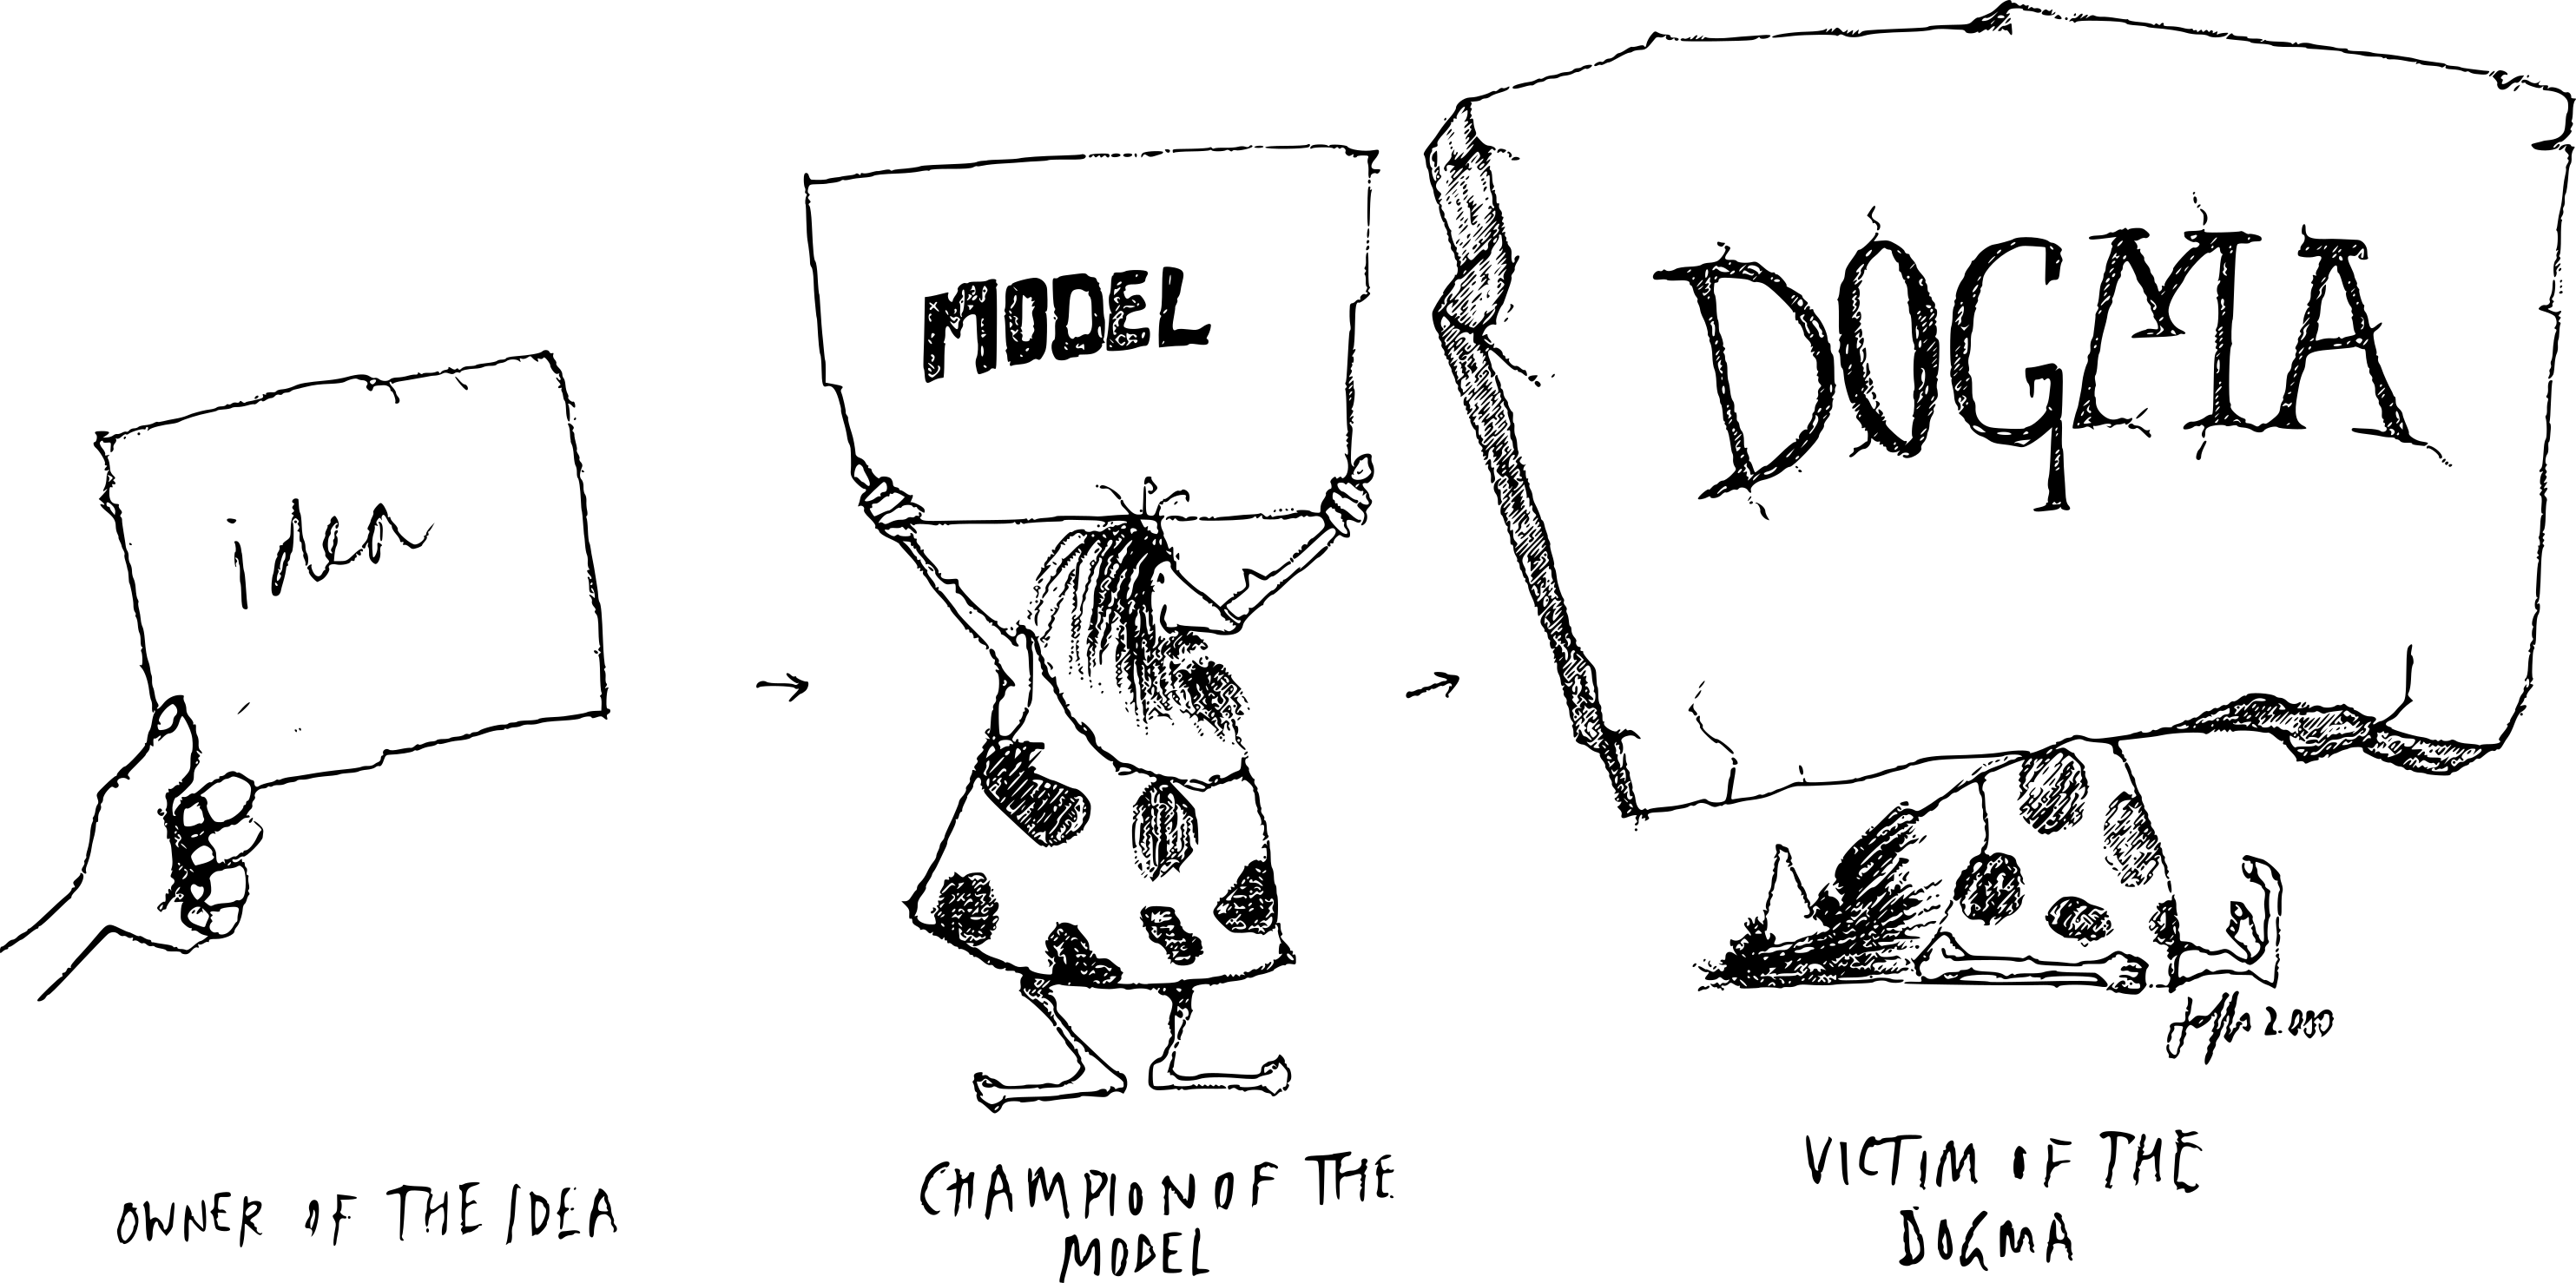
\includegraphics[width=\linewidth]{ch.discussion/imgs/dogma.png}
    \caption{\textbf{The phylotypic stage as a (crushing) scientific dogma?} \cite{Caveman2000}}
    \label{fig:dogma}
\end{figure}

These examples highlight the dogmatic belief in the (non)existence of a phylotypic stage, and a potential reluctance to sincerely interact with each other's works. On top of that, in \textbf{Chapters 4 and 5}, I discuss the methodological issues in comparative analyses concerning the phylotypic stage. The root problem is that the phylotypic stage and its related models are ill-defined, and as a consequence, there is a lack of appropriate (statistical) controls in these studies. Is temporal conservation in these models present in comparisons within and between phyla? And is temporal conservation already observable when comparing a species against itself? By systematically addressing these ambiguities in previous studies through within-species, between-species, and between-phyla comparisons I show examples where the conclusions are not supported by the data. To summarize my main findings:
\begin{itemize}
    \item The transcriptomic hourglass-like pattern between zebrafish and frogs\cite{marletaz2018} can be explained by within-species correlations alone.
    \item The transcriptomic between-phyla inverse hourglass pattern\cite{Levin2016} is a statistical artifact and can be reproduced by simulated data with no specific temporal conservation.
    \item The pattern of cell type proportion similarity between rabbits and mice\cite{Mayshar2023} can be explained by discontinuous temporal sampling.
    \item The \textit{Drosophila} enhancer conservation re-analysis results in a "mid-developmental" stage of maximum similarity, albeit at a different point than found by the original authors. Moreover, in \textbf{Chapter 4} I highlight additional problems with the binarization of enhancers, and as such I do not endorse this methodology.
    \item  The morphological within-phylum inverse hourglass pattern is caused by edge effects and can be reproduced by simulated data with no specific temporal conservation.
\end{itemize}
\noindent
The null model for evolutionary embryonic development would be that there is no specific stage of higher or lower temporal conservation. Altogether, I have found little evidence to reject the null hypothesis of constant temporal conservation based on quantitative data, and thus see no reason to suppor a (molecular) phylotypic stage.

Moreover, in \textbf{Chapter 4} I discuss further ambiguities in the models of the phylotypic stage. If a molecular phylotypic stage would exist, which genetic features are expected to be conserved and which are not? The original observation that vertebrate embryos, perhaps, look more like each other \textit{externally} at certain points in development, says little about the whole-embryo molecular basis for it. While the morphological observations of Haeckel are almost 200 years old, there have been only two quantitative studies about the morphological phylotypic stage, and these two studies were in direct contradiction with each other. Instead, there appears to be a pursuit to find new (quantitative) methodologies that produce a more straight-forward confirmation of the existence of the phylotypic stage, such as embryonic lethality\cite{Uchida2018},  DNA sequence conservation\cite{Piasecka2013,Quint2012,Liu2021} and activation order\cite{Uesaka2019}, cell type proportion\cite{Mayshar2023}, and whole-transcriptome similarity\cite{Piasecka2013,Irie2011,marletaz2018,Liu2020,Leong2021,PerezPosada2022,Kalinka2010}, with little published effort to integrate these results across studies. Of these methodologies, the whole-embryo transcriptome has become the most popular method to asses quantitative similarity. The implicit justification for this is that transcriptomics is an unbiased way to study genes during development. Even assuming the phylotypic stage exists, why would we expect to be able to measure such a complex phenomenon with such relatively crude methods as observational studies and whole embryo sequencing? 

Throughout scientific history, certain theories, such as taxonomic phyla and the phylotypic stage, have evolved from initial concepts into widely accepted truths, creating a demand for a molecular explanation along the way. However, a fundamental issue arises from the loose and ambiguous definitions on which these theories are based, leading to their lack of predictive power and falsifiability, rendering them, by Popperian standards, non-scientific in nature. For instance, the concept of phyla hinges on the notion that animals sharing a common basic body plan are part of the same phylum, yet paradoxically, the basic body plan is defined as the morphological characteristics shared by all animals within the same phyla\cite{BUDD2000,scholtz2004bauplane}. The definition of the phylotypic stage is similarly ambiguous. Historically, the pharyngula stage\cite{BALLARD1981}, early somite embryo\cite{Alberch1993}, and the tail bud stage \cite{Slack1993} have all been proposed as the vertebrate phylotypic stage. In quantitative studies, the choice of definition in turn depends on which stage exhibits the highest quantitative conservation. Consequently, the pharyngula \cite{Irie2011,marletaz2018}, the early somite embryo \cite{DomazetLoso2010}, or simply the stage(s) with the highest conservation metric\cite{Kalinka2010,Cordero2020} have all been identified as phylotypic stages. In conclusion, our current approach to studying the phylotypic stage, where we selectively include definitions and ignore non-conforming results, is not only wrong, but also not useful.

\section{The technical debt of bioinformatics}

The complexity of molecular biological systems naturally makes their (bioinformatic) analysis a complex task as well. Their analysis is further complicated by the continuous addition of new insights, which leads to updated methodologies and analytical approaches, keeping the field of bioinformatics in a state of perpetual change. Often, in the rush to generate new insights, tools are developed quickly, leading to solutions that, while functional, may not fully capture the nuances of the underlying biology. In turn, the bioinformatics community builds upon these tools, perpetuating their inefficiencies. Eventually, the burden of these suboptimal solutions becomes untenable, which requires major revisions of the original methodology. In software development, this concept is known as technical debt. Technical debt, similar to financial debt, means that shortcuts taken today must be paid back in the future, often at a greater cost. I believe that in the field of bioinformatics, the technical debt has become so large that it has become prohibitive for most analyses.

A significant source of technical debt exists in the data structures bioinformatics uses. During my doctoral studies, I have extensively made use of positional genomic formats such as the GFF and GTF formats, the FASTA format, and Position Weight Matrices (PWMs). The General Feature Format (GFF), and its derived Gene Transfer Format (GTF) are formats that are not fit for their use anymore. The GFF and GTF format specify genomic features and their locations, where each line represents a feature and the columns are different attributes. One of these columns indicates the position position of the feature in a one-indexed coordinate system. This differs from the widely held view, albeit slightly subjective, that zero-indexing is the norm for coordinate systems\cite{utexasEWDijkstra}. This makes one-off errors between these formats and other positional formats, such as BED, easy to make. Moreover, as our understanding of genes got more complex, so did their subsequent analysis. This meant that it became necessary to express more complex relationships between features within these GFF and GTF files. Flat formats such as GTF and GFF can not naturally represent this, yet the newer GFF and GTF formats now specify these relationships in a \say{attribute-value} column. This has made these formats less suitable to be parsed line-by-line, something for which they were originally designed. Even the first sentence of the GFF3 format starts disagreeing with its own design; \say{although there are many richer ways of representing genomic features ..., the stubborn persistence ... of ad-hoc tab-delimited flat file formats declares the bioinformatics community's need for a simple format that can be modified with a text editor and processed with shell tools like grep}\cite{GFFformat}. Moreover, the unstructured manner in which these new formats were released resulted in multiple incompatible dialects. The frustration of the field about the GFF and GTF formats is best illustrated by a Tweet from Lior Pachter, where he asked if there is a citation for the GTF format. The most popular response covered the collective frustration of the field, stating \say{Ain’t no one gonna take responsibility for that mess}\cite{Pachter_2023}. A transition to a relational data format, capable of adequately handling the increasing complexity and relationships in genomic data, seems not only logical but inevitable.

FASTA is a text-based format that represents nucleotide sequences or amino acid sequences, in which nucleotides are represented using a single-letter\cite{Lipman1985}. Single nucleotide polymorphisms are defined by their IUPAC codes, but uncertainties longer than a single nucleotide (haplotypes) can not be naturally represented. This problem is solved by appending alternative sequences to the file. These sequences can then be selectively used in the downstream analysis. However, bwa mem(2)\cite{bwamem,bwamem2}, and Illumina Dragen are the only genomic aligners that support this natively. Consequently, despite alternative regions being part of the human genome since 2013, structural variation is typically overlooked in studies. Moreover, for some researchers the difference between a primary assembly (no alternative sequences) and a toplevel assembly (includes alternative sequences) might not be clear, causing them to align their reads against a toplevel assembly. This results in many multimapped reads, and consequently a low coverage in these regions. Thus, the limitations of FASTA in representing haplotypes highlight the necessity for adopting more sophisticated file formats like pangenomes\cite{Li2020}, which represent haplotypes more effectively.

Finally, PWMs quantify the log-likelihood of each nucleotide's presence in a motif. While PWMs are straightforward to understand and visually interpret, they oversimplify transcription factor binding by assuming that nucleotides within a binding site act independently\cite{Zuo2014,Jolma2015,Inukai2017}. Higher-order structures, such as DNA methylation and DNA shape, can not be naturally represented in PWMs. As a consequence, motif databases consist of numerous nearly identical PWMs, one motif for each dependence between nucleotides. A notable example of this is the SCENIC+ motif database\cite{BravoGonzlezBlas2023}, which claims to have compiled the largest collection of motifs to date, containing over 30,000 \say{unique} motifs. However, the motifs in this database are distributed among approximately 3,000 TFs between humans, mice, and fruit flies, demonstrating a considerable amount of redundancy. Alternatives, such as graph-based PWMs\cite{Siebert2016} and neural networks\cite{Novakovsky2023,https://doi.org/10.48550/arxiv.1704.02685}, do incorporate dependence between nucleotides and as such offer a more complete understanding of TF binding.

Whilst the outdated data formats represent a more systematic and difficult-to-solve technical debt, there is also a considerable amount of low-effort technical debt. This includes the use of old assemblies, unresolved bugs, and unoptimized software. For example, in 2023, Google Scholar identified 7,630 publications that used the older hg19 or GRCh37 genome assemblies (released in 2009), while there were only 8,960 publications that used the newer hg38 or GRCh38 assemblies (released in 2013). Notably, the T2T-CHM13 assembly (released in 2022) has only been mentioned in 222 publications in 2023. Whilst I recognize that using an older genome version might be preferable in comparisons to previously analyzed data or databases, not updating your assembly perpetuates the use of outdated versions. Not surprisingly, a newer genome assembly results in more accurate and new discoveries\cite{Aganezov2022,Pan2019}. 

Another easily addressed problem is resolving identified bugs in popular software. For example, MACS2 is one of the most popular tools in the field of regulatory genomics and is used to discover enriched regions in the genome. MACS2 has been cited more than 14,000 times\cite{Zhang2008}. Despite its popularity, it contains some unexpected default settings. The recommended way to use MACS2 in the case of ATAC-seq discards all mates from paired-end data, effectively removing half of the cleavage information\cite{Gaspar2018}. Whilst this can be overcome by some specific processing on the user side, most users are not aware of this setting, resulting in suboptimal peak sets in presumably the majority of ATAC-seq studies that use MACS2. Similarly, a popular toolkit for the analysis of single-cell data, Seurat, contains a particularly painful bug. Its implementation of the log fold change calculates the log of the means (as opposed to the mean of the logs), which makes it sensitive to outliers. This results in unexpected log fold changes and vastly different outcomes depending on whether one used Seurat or any alternative tool such as Scanpy for their analysis. The bug was reported in November 2022, got an incomplete fix in March 2023, and as yet, January 2024, has not been fixed\cite{WatsonHaigh}. Seurat has been cited more than 8,000 times. 

Finally, most software is usually poorly optimized, especially in the field of single-cell analyses, taking days to run and requiring enormous amounts of memory\cite{Pratapa_2020}. The usual solution in the field to this problem is, surprisingly, not to improve the software implementation, but instead to increase the hardware capabilities. For instance, an ex-colleague of mine requested a massive 4TB of RAM for his computer at his new position. This practice not only causes enormous computational waste but also creates a substantial barrier to researchers from labs without such resources.

A personal example of how technical debt directly affected my doctoral studies is through the Sequence Read Archive (SRA). The SRA is a public repository that serves as a centralized archive for storing and sharing high-throughput sequencing data. The SRA has been essential for my doctoral studies, as I have relied solely on public data. For \textbf{Chapter 6}, I aimed to download all available human H3K27ac data (+/- 12,000 samples) from the SRA as a reference database. Processing these samples meant that I had to download 20TB from the SRA and spent approximately 300,000 CPU hours processing them on Cartesius, costing an enormous amount of computational resources and emitting an estimated one-and-a-half tonnes of CO\textsubscript{2}\footnote[2]{300,000 CPU hours, spread over the 8 cores of an Intel Xeon Processor E5-2670 uses 115W\cite{intelIntelXeon}, which results in a total estimated energy usage of 4312 kWh. The production of one kWh emitted an average of 369 grams of CO\textsubscript{2} in the Netherlands in 2019\cite{CO2}, which in turn leads to a total CO\textsubscript{2} production of 1591 kg. Furthermore, this calculation ignores the significant electricity usage of data transfer and working memory.}. In the analysis that followed, however, it turned out that obtaining sample annotations, such as tissue or cell type, is challenging due to the lack of standardized metadata on the SRA. Third-party tools like MetaSRA\cite{Bernstein2017}, and PredictMEE\cite{Klie2021} have been developed to automatically infer this metadata but ultimately failed to provide accurate results. In the end, I decided to discard the experiment, wasting an enormous amount of resources. Whilst the wasted computational resources could have been avoided by a pilot study on my side, an unstructured SRA is an enormous wasted opportunity. My experience with the SRA is exemplary of a broader trend in big data bioinformatics research, where ENCODE is preferred over the SRA despite its smaller size, in part because it offers structured metadata.

Not only is the SRA lacking crucial metadata, but its sra-tools, a toolkit for interacting programmatically with the SRA are particularly hard to use. As a consequence, many alternative tools have been developed for downloading data from the SRA, such as the SRA-explorer\cite{sraexplorer}, pysradb\cite{Choudhary2019}, FetchFastQ\cite{galvez2022metadata}, nf-core/fetchngs\cite{fetchngs}, parallel-fastq-dump\cite{parallelfastq}, and finally our download-fastq workflow of seq2science\cite{seq2science} (\textbf{Chapter 3}). The poor implementation of the sra-tools results in additional and unnecessary work, wasting the time and resources of third-party researchers. Similarly, the submission of new sequencing data is notoriously complicated which has even led others to develop tools to streamline the upload process\cite{Quiones2020}. 

I consider all of the aforementioned examples, like inadequate data formats, outdated assemblies, unresolved bugs, and the SRA, as technical debt. Addressing these issues is crucial for advancing the field; it's not a matter of whether they should be addressed, but rather how and when. Even though addressing some of these problems will require substantial effort, postponing their resolution will not simplify the task. Moreover, delaying the resolution hinders all current and future analyses with a less efficient process. In my opinion, there are three main reasons for the widespread technical debt in bioinformatics; (i) insufficient incentives to maintain and develop high-quality software, (ii) the lack of interdepartmental software collaborations, and (iii) the lack of formal bioinformatics training.

It appears that writing high-quality software is not incentivized, although frankly, I have little personal experience with this part of science. Typically, the end product of an analysis is a scientific publication, and in the rush to generate new insights, software, and tools emerge as byproducts. Consequently, their design rarely prioritizes adaptability or user-friendliness for broader applications. This problem is reinforced by the fact that funding decisions are based predominantly on the impact of previous research and the novelty of the newly proposed work. Prominent grant opportunities like the NWO Veni, Vidi, and Vici grants, EMBO postdoctoral fellowships, and Marie Skłodowska-Curie Postdoctoral Fellowships all emphasize the importance of innovative applications. This emphasis on innovation creates a strong selection pressure for researchers doing novel work, inadvertently disadvantaging researchers dedicated to maintaining and enhancing existing software. While maintaining one's own software can potentially lead to increased citations and, by extension, improved funding prospects, this is not the case for the maintenance of crucial third-party software. The current funding system undervalues the maintenance of scientific software in bioinformatics, which by extension perpetuates its technical debt.

A different cause for technical debt is the fact that most tools are developed independently, most of the time by a single doctoral student or postdoc. This has two major downsides. The first is that the maintenance of tools depends on individuals. If someone decides to leave academia, their tools, how useful they might be, will soon become obsolete as no one will maintain them. A clear example is the dissolution of the \say{van Heeringen} group, where soon tools such as genomepy\cite{Frlich2023}, gimmemotifs\cite{Bruse_2018}, ANANSE\cite{Xu_2020}, SCEPIA (\textbf{Chapter 6}), seq2science\cite{seq2science} (\textbf{Chapter 3}), and qnorm\cite{qnorm} will become outdated as they will no longer be maintained. Second, as most tools are a byproduct of an analysis, they are often highly specialized for specific tasks. This, in turn, leads to many near-identical tools that solve similar problems, for example, all the different SRA FASTQ downloading tools. This is in stark contrast to the formulation of the SAM/BAM format\cite{Li2009} and the subsequent implementation of HTSLIB\cite{Bonfield2021}. The SAM/BAM formats are the \textit{de facto} standard for genomic alignments in the field, with the HTSLIB as the library to work with these files. This project was led by the 1000 Genomes project, which means that numerous bioinformaticians were and still are involved in their design. This guarantees that the SAM/BAM format is useful for a wide range of different applications. Moreover, an important detail is that the developers of the SAM/BAM format and HTSLIB are researchers and using their own implementations, something I suspect that the developers of the SRA are not. This guarantees that the developers continuously test their own implementations for ease of use and correctness. Even though HTSLIB was started over a decade ago, it is still receiving regular updates. 

Finally, as the field of bioinformatics continues to grow, the demand for skilled bioinformaticians is outpacing the current supply. This dynamic has led to an inclusive approach in the field, where biologists from various backgrounds are engaging in bioinformatics analyses. This inclusivity is exemplified by projects like Galaxy\cite{galaxy}, which have been instrumental in making bioinformatics accessible. However, whilst this inclusivity is beneficial, we should not neglect the need for specialized skills in certain areas of bioinformatics. For instance, the development of tools and file formats, as well as the execution of complex analyses, often require a deeper understanding of programming, statistics, and modeling. A telling example of the lack of formal training is the widespread use of Excel in bioinformatics analysis. Excel notoriously used to mangle gene names\cite{Zeeberg2004}, for example, the gene alias \textit{SEPT1} was automatically converted into September 1. Consequently, approximately $30\%$ of studies report these mangled gene aliases in their supplementary data\cite{Abeysooriya2021}! In 2020 the HGNC opted to change 27 gene names to avoid Excel name mangling, and the \textit{SEPT1} alias became \textit{SEPTIN1}. Thus, while inclusivity solves the demand for bioinformaticians in the short term, the intricacies of biology and bioinformatics do also demand more formally trained bioinformaticians.

In conclusion, addressing the technical debt in bioinformatics is crucial for the advancement of the field. This requires a collective effort to update and refine data representation models, resolve software bugs, and optimize existing tools. Additionally, a fundamental shift in the scientific culture of biology is needed, where the development and maintenance of software are given the same importance as novel research. This shift should include incentivizing high-quality software development, fostering interdepartmental collaborations, and emphasizing the need for formal training in bioinformatics. Only through these measures can we ensure that bioinformatics research remains reliable, accurate, and efficient. 

\section{Concluding Remarks}

Transcription is a highly complex process, which depends on numerous factors such as chromatin context and transcription factor gene expression. The regulation of transcription is dynamic and changes throughout (embryonic) development, and is prone to changes through evolution. To study this phenomenon, experimental biologists have generated enormous amounts of data, which is typically analyzed by bioinformaticians and computational biologists. In this thesis I propose three improvements to gene regulatory network inference; the use of multiple omics, the use of single-cell data over bulk sequencing, and the use of foundation models. Additionally, I introduce two computational tools that aid in the investigation of transcription regulation. Seq2science is an end-to-end functional genomics preprocessing tool, and SCEPIA is a tool that facilitates the linking of single-cell transcriptomic information to an extensive database of chromatin context to improve motif activity inference. Furthermore, in this thesis, I present my findings on the phylotypic stage, a stage that is supposedly highly conserved between species. I explain how its many definitions are ambiguous, which leads to unsupported conclusions from the data. Altogether, this thesis provides computational perspectives on transcription regulation throughout evolution and development. 
